\documentclass[14pt]{article}
\usepackage{geometry}
\usepackage[utf8]{inputenc}
\usepackage{cmap}
\usepackage[russian]{babel}
\usepackage{textcomp}
\usepackage{indentfirst}
\usepackage{amssymb}
\usepackage{graphicx}
\usepackage{lipsum}
\usepackage{setspace}
\usepackage{extsizes}
\usepackage{enumitem}
\usepackage{tabularx}
\usepackage{amsmath}
\usepackage{tocloft}
\usepackage{minted}
\usepackage[colorlinks=true,urlcolor=blue,linkcolor=]{hyperref}

\usepackage{graphicx}
\graphicspath{ {./images/} }

\renewcommand{\cftsecleader}{\cftdotfill{\cftdotsep}}
\renewcommand{\cfttoctitlefont}{\LARGE\bfseries}
% Начало блока кода, который позволяет включить section* в оглавление
\usepackage{etoolbox}
\makeatletter
\newcommand\mysection[1]{%
	  \addcontentsline{toc}{section}{#1}%
	  \section*{#1}%
}
\makeatother

\makeatletter
\newcommand\mysubsection[1]{%
	  \addcontentsline{toc}{subsection}{#1}%
	  \subsection*{#1}%
}
\makeatother

\makeatletter
\newcommand\mysubsubsection[1]{%
	  \addcontentsline{toc}{subsubsection}{#1}%
	  \subsubsection*{#1}%
}
\makeatother
% Конец блока кода

\usepackage{titlesec}
\titleformat*{\section}{\LARGE\bfseries\centering}
\titleformat*{\subsection}{\Large\it}
\usepackage{pgfplots}

\newcolumntype{Y}{>{\centering\arraybackslash}X}

\begin{document}
\newgeometry{top=0.1in,bottom=0in,right=0.1in,left=0.1in}
\begin{spacing}{1}
\begin{center}
	\makebox[\linewidth][s]{МИНИСТЕРСТВО НАУКИ И ВЫСШЕГО ОБРАЗОВАНИЯ РОССИЙСКОЙ ФЕДЕРАЦИИ} \\
	\vspace{5mm}
	ФЕДЕРАЛЬНОЕ ГОСУДАРСТВЕННОЕ АВТОНОМНОЕ ОБРАЗОВАТЕЛЬНОЕ \\ УЧРЕЖДЕНИЕ ВЫСШЕГО ОБРАЗОВАНИЯ  \\
	\guillemotleft Национальный исследовательский университет ИТМО\guillemotright \\
	\vspace{5mm}
	ФАКУЛЬТЕТ ПРОГРАММНОЙ ИНЖЕНЕРИИ И КОМПЬЮТЕРНОЙ ТЕХНИКИ
	\vspace{60mm}
	
	{\bf \LARGE ЛАБОРАТОРНАЯ РАБОТА №1} \\
	{ \Large по дисциплине \\
	\guillemotleft Системы искусственного интелекта \guillemotright \\}
\end{center}
\vspace{50mm}

\begin{flushright}
	{\it \textbf{Выполнил работу:}}\\
	Студент группы P3318 \\
	Рамеев Тимур Ильгизович \\
	{\it \textbf{Преподаватель:}}\\
	Авдюшина Анна\\
	Евгеньевна \\
\end{flushright}
\vspace{18mm}
\end{spacing}
\begin{center}
    Санкт-Петербург  2024
\end{center}

\newgeometry{a4paper, top=10mm, bottom=20mm, left=20mm, right=10mm}

\newpage
\begin{center}
	\tableofcontents 
\end{center}
\setcounter{page}{1}

\newpage
\mysection{Цель}
	Знакомство с базами знаний и онтологиями, языком Prolog и редактором онтологий Protege.
\mysection{Анализ требований}
Система должна предоставлять  следующий функционал:
	\begin{enumerate}[itemsep=-5pt]
		\item На основе предпочтений (любимого времени года,  позиции и роли персонажа) советовать, ранжировать персонажей и предлагать наиболее подходящих для выбора
		\item Выводить подробную информацию о заданном персонаже, а при некорректном вводе выводить список всех имеющихся персонажей
		\item Выводить подробную информацию о заданной территории, а при некорректном вводе выводить список всех имеющихся территорий
	\end{enumerate}
\mysection{Основные концепции и инструменты}
	В основе баз знаний лежат факты и правила. Факты представляют из себя верные отношения между сущностями, а правила - способы порождения новых фактов из имеющихся. \\
	Для использования базы знаний необходимо задать цель - неизвестную переменную в предикате, которую база попытается подобрать так, чтобы предикат был верен. \\
	Язык Prolog позволяет описать базу занний декларативно. В нем можно описать факты - верные предикаты с полными аргументами, а также задать аналоги функций - правила. \\
	В проекте мы не будем работать с Prolog напрямую, а будем использовать интерпретатор pyswip.
\mysection{Реализация системы ИИ}
\mysubsection{Описание базы знаний}
	База знаний, написанная на языке Prolog, содержит информацию о персонажах вселенной League Of Legends. В ней описаны класс персонажа, его роль на карте, место обитания (по лору), а также враждебные отношения между персонажами (по лору).
	Также база знаний содержит следующие правила:
	\begin{enumerate}[itemsep=-5pt]
		\item Правило для поиска персонажей с одной территории
		\item Правило для поиска персонажей с одинаковой ролью
		\item Правило, ищущее всех топеров-стрелков
		\item Правило для поиска войны между территориями
		\item Правило для поиска врагов с одинаковой ролью на карте
		\item Правило для поиска друзей (Территории с общим врагом без войны друг с другом)
	\end{enumerate}

\newpage
\mysection{Запросы к базе знаний}
	Помимо базы знаний, были написаны несколько запросов к ней, для демонстрации ее работы:
	\begin{enumerate}[itemsep=-5pt]
		\item Посмотреть всех убийц
		\item Посмотреть с какой территории песонаж Трэш
		\item Посмтотреть есть ли враги у Ка'Зикса
		\item Посмтотреть магов из Бандл-Сити, играющих на топе или на миде
		\item Посмотреть всех врагов Ноксуса
		\item Посмотреть всех воинов и убийц играющих против магов на одной позиции
	\end{enumerate}


\mysection{Программная часть}
\mysubsection{База знаний}
\begin{minted}[mathescape, linenos]{prolog}
% Роль персонажа
tank(tarik).
tank(trash).
tank(braum).
wizard(zerat).
wizard(ari).
wizard(sweyn).
wizard(reykan).
wizard(veigar).
wizard(luxe).
warrior(vai).
warrior(viego).
warrior(darius).
warrior(saylas).
warrior(warwick).
warrior(garen).
killer(khaZix).
killer(rengar).
killer(pyke).
killer(zed).
killer(ekko).
killer(katarina).
shooter(timo).
shooter(ashe).
shooter(senna).
shooter(lucian).
shooter(dreivan).
shooter(jinx).

% Родина персонажа ( по лору )
homeland(shadowyIslands, lucian).
homeland(shadowyIslands, senna).
homeland(shadowyIslands, viego).
homeland(shadowyIslands, trash).
homeland(gapingHole, khaZix).
homeland(bildgwater, pyke).
homeland(ionia, zed).
homeland(ionia, rengar).
homeland(ionia, reykan).
homeland(nocsus, sweyn).
homeland(nocsus, dreivan).
homeland(nocsus, darius).
homeland(nocsus, katarina).
homeland(zaun, jinx).
homeland(zaun, vai).
homeland(zaun, ekko).
homeland(zaun, warwick).
homeland(demasiya, luxe).
homeland(demasiya, garen).
homeland(freljord, saylas).
homeland(freljord, ashe).
homeland(freljord, braum).
homeland(targon, tarik).
homeland(bandlCity, veigar).
homeland(bandlCity, timo).
homeland(bandlCity, ari).
homeland(shurima, zerat).


% Место отыгрыша на карте (Некорректно немного получилось)
role(carry, lucian).
role(support, trash).
role(support, senna).
role(jungle, viego).
role(jungle, khaZix).
role(support, pyke).
role(mid, zed).
role(jungle, rengar).
role(support, reykan).
role(support, sweyn).
role(carry, dreivan).
role(top, darius).
role(carry, jinx).
role(jungle, vai).
role(jungle, ekko).
role(jungle, warwick).
role(mid, luxe).
role(top, garen).
role(mid, saylas).
role(carry, ashe).
role(support, braum).
role(support, tarik).
role(mid, veigar).
role(top, timo).
role(mid, ari).
role(mid, zerat).
role(mid, katarina).

% Враги (по лору )
enemies(khaZix, rengar).
enemies(saylas, garen).
enemies(garen, darius).
enemies(katarina, ari).
enemies(timo, pyke).
enemies(senna, trash).
enemies(senna, viego).
enemies(lucian, trash).
enemies(lucian, viego).
enemies(jinx, vai).

% Персонажи с одной территории
countrymans(X, Y) :- homeland(Z, X), homeland(H, Y), Z = H, X \= Y.

% Персонажи с одинаковой ролью
sameRoles(X, Y) :- role(Z, X), role(H, Y), Z = H, X \= Y.

% Топеры-стрелки
topShooters(X) :- role(top, X), shooter(X).

% Войны между территориями
wars(X, Y) :- homeland(X, Z), homeland(Y, H), (enemies(Z, H); enemies(H, Z)), X \= Y.

% Враги с одинаковой позицией в игре
sameEnemiesByRole(X, Y) :- role(Z, X), role(H, Y), (enemies(X, Y); enemies(Y, X)), X \= Y, Z = H.

% Друзья (Территории с общим врагом без войны друг с другом)
friends(X, Y) :- wars(X, Z), wars(Y, Z), not(wars(X, Y)), X \= Y.
\end{minted}

\mysubsection{Запросы к базе знаний}
\begin{minted}[mathescape, linenos]{prolog}
% посмотреть всех убийц
killer(X).

% посмотреть с какой территории Треш
homeland(X,trash).

% посмотреть, есть ли враги у казикса
enemies(khaZix, _); enemies(_, khaZix).

% посмотреть магов из Бандл-Сити, играющих на топе или на миде
wizard(X), homeland(bandlCity, X), (role(top, X); role(mid, X)).

% посмотреть всех врагов Ноксуса
{Z}/(wars(nocsus, Y), homeland(Y, Z)).

% посмотреть всех воинов и убийц играющих против магов на одной линии
(killer(X); warrior(X)), wizard(Y), role(Role, X), role(Role, Y).
\end{minted}

\mysubsection{Консольное приложение}
Написано на языке Python
\begin{center}
\begin{minted}[mathescape, linenos]{python}
from pyswip import Prolog

def start_dialog():
    while True:
        print("Привет! Меня зовут БОБ! Я - база знаний по игре League of Legends. Выбери одну из следующих опций:")
        print("a) Подобрать персонажа")
        print("b) Узнать информацию о персонаже")
        print("c) Посмотреть друзей и врагов выбранной территории")
        print("d) Выход")
        option = input().strip()
        if option == "a":
            find_character_manager()
        elif option == "b":
            find_info_character_manager()
        elif option == "c":
            find_info_territory_manager()
        elif option == "d":
            break
        else:
            print("Похоже я вас не понимаю, пожалуйста попробуйте еще раз")


def find_info_territory_manager():
    print("Вы выбрали опцию \"Посмотреть друзей и врагов выбранной территории\". Отлично! Введите наименование территории")
    name_of_territory = input()
    wars = [x['X'] for x in list(prolog.query(f'wars(X, {name_of_territory})'))]
    friends = [x['X'] for x in list(prolog.query(f'friends(X, {name_of_territory})'))]
    valid_name = list(prolog.query(f'homeland({name_of_territory}, X)'))
    if len(valid_name) > 0:
        print("Итак, я нашел некоторую информацию об этой территории:")
        print(f"Наименование территории: {name_of_territory}")
        print(f"Враждебные территории: {wars}")
        print(f"Союзные территории: {friends}")
    else:
        print("Извините я не нашел такой территории, вот, на всякий случай, список всех территорий, о которых я что-то знаю")
        all_lands =list(set(x['X'] for x in list(prolog.query("homeland(X, Y)"))))
        for i in range(1, len(all_lands) + 1):
            print(i, " : ", all_lands[i - 1])

def find_info_character_manager():
    print("Вы выбрали опцию \"Узнать информацию о песонаже\". Отлично! Введите имя персонажа, о котором хотите узнать")
    name_of_character = input()
    homeland = list(prolog.query(f'homeland(X, {name_of_character})'))
    role = list(prolog.query(f'role(X, {name_of_character})'))
    position = list(prolog.query(f'position(X, {name_of_character})'))
    enemies = list(prolog.query(f'enemies(X, {name_of_character}); enemies({name_of_character}, X)'))
    countrymans = list(prolog.query(f'countrymans(X, {name_of_character})'))
    if len(homeland) == 1:
        print("Итак, я нашел некоторую информацию об этом парнише:")
        print(f"Имя персонажа: {name_of_character}")
        print(f"Родина персонажа: {homeland[0]['X']}")
        print(f"Роль персонажа: {role[0]['X']}")
        print(f"Позиция персонажа: {position[0]['X']}")
        if len(enemies) > 0:
            print("Враги персонажа: ", [x['X'] for x in enemies])
        else:
            print("У персонажа отсутствуют враги")
        if len(countrymans) > 0:
            print("Соотечественники персонажа: ", [x['X'] for x in countrymans])
        else:
            print("У персонажа отсутствуют соотечественники")
    else:
        print("Извините, я не нашел такого персонажа, вот, на всякий случай, список всех песонажаей, про которых я что-то знаю:")
        all_chars = [x['X'] for x in list(prolog.query("character(X)"))]
        for i in range(1, len(all_chars) + 1):
            print(i, " : ", all_chars[i - 1])


def find_character_manager():
    while True:
        try:
            print("Вы выбрали опцию \"Подобрать персонажа\". Отлично! Сейчас я задам Вам ряд вопросов, на основе которых, приму решение о том, какой персонаж вам подходит больше всего")
            result_list = homeland_choise() + role_choise() + position_choise()
            result_dict = {1 : set(), 2 : set(), 3 : set()}
            for item in result_list:
                result_dict[result_list.count(item)].add(item)
            
            print("Итак, вот персонажи, которых я для Вас нашел:")
            print("Наилучшая синергия:", result_dict[3])
            print("Вы неплохо поладите:", result_dict[2])
            print("Будет тяжеловато освоиться:", result_dict[1])
            print("Остальных персонажей крайне не рекомендую. Удачи, боец!")
            break
        except Exception as unrecognized_input:
            print("Похоже я вас не понимаю, пожалуйста попробуйте еще раз")
            continue
    
    
def homeland_choise():
    print("Какое время года Вам нравится больше всего?")
    print("a) Зима")
    print("b) Весна")
    print("c) Лето")
    print("d) Осень")
    season = input().strip()
    if season == "a":
        season = "winter"
    elif season == "b":
        season = "spring"
    elif season == "c":
        season = "summer"
    elif season == "d":
        season = "autumn"
    else:
        raise Exception
    return [x['Y'] for x in list(prolog.query(f'homeland(X, Y), season({season}, X)'))]

def role_choise():
    print("Какая роль вам нравится больше всего?")
    print("a) Убийца")
    print("b) Танк")
    print("c) Маг")
    print("d) Стрелок")
    print("e) Воин")
    role = input().strip()
    if role == "a":
        role = "killer"
    elif role == "b":
        role = "tank"
    elif role == "c":
        role = "wizard"
    elif role == "d":
        role = "shooter"
    elif role == "e":
        role = "warrior"
    else:
        raise Exception
    return [x['Y'] for x in list(prolog.query(f'role({role}, Y)'))]

def position_choise():
    print("На какой позиции на карте вы бы хотили отыгрывать?")
    print("a) Топ")
    print("b) Керри")
    print("c) Саппорт")
    print("d) Лес")
    print("e) Мид")
    position = input().strip()
    if position == "a":
        position = "top"
    elif position == "b":
        position = "carry"
    elif position == "c":
        position = "support"
    elif position == "d":
        position = "jungle"
    elif position == "e":
        position = "mid"
    else:
        raise Exception
    return [x['Y'] for x in list(prolog.query(f'position({position}, Y)'))]

prolog = Prolog()
prolog.consult("Lab1/knowledgeBase.pl")
start_dialog()
\end{minted}
\end{center}

\mysection{Онтологический граф}
\begin{center}
	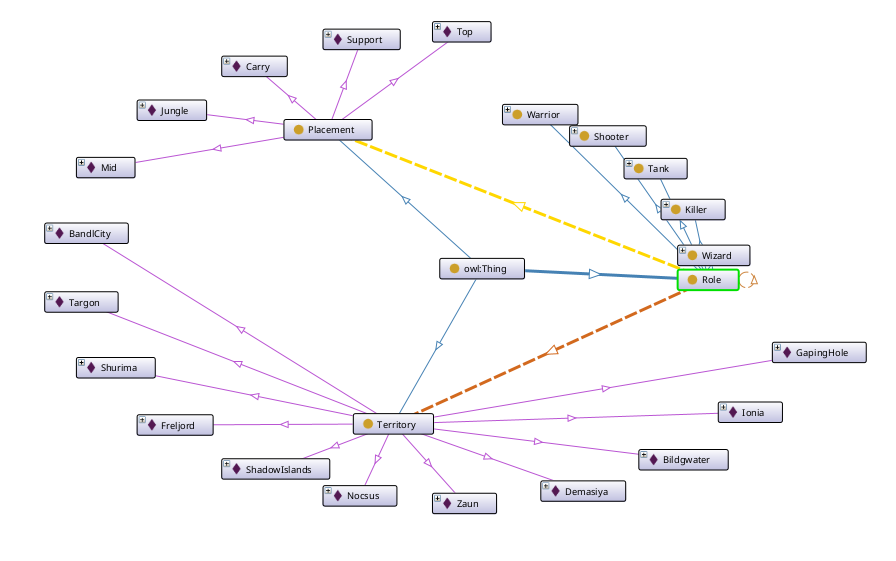
\includegraphics[scale=0.6]{onto_graph}
\end{center}

\mysection{Объектные свойства}
\begin{center}
	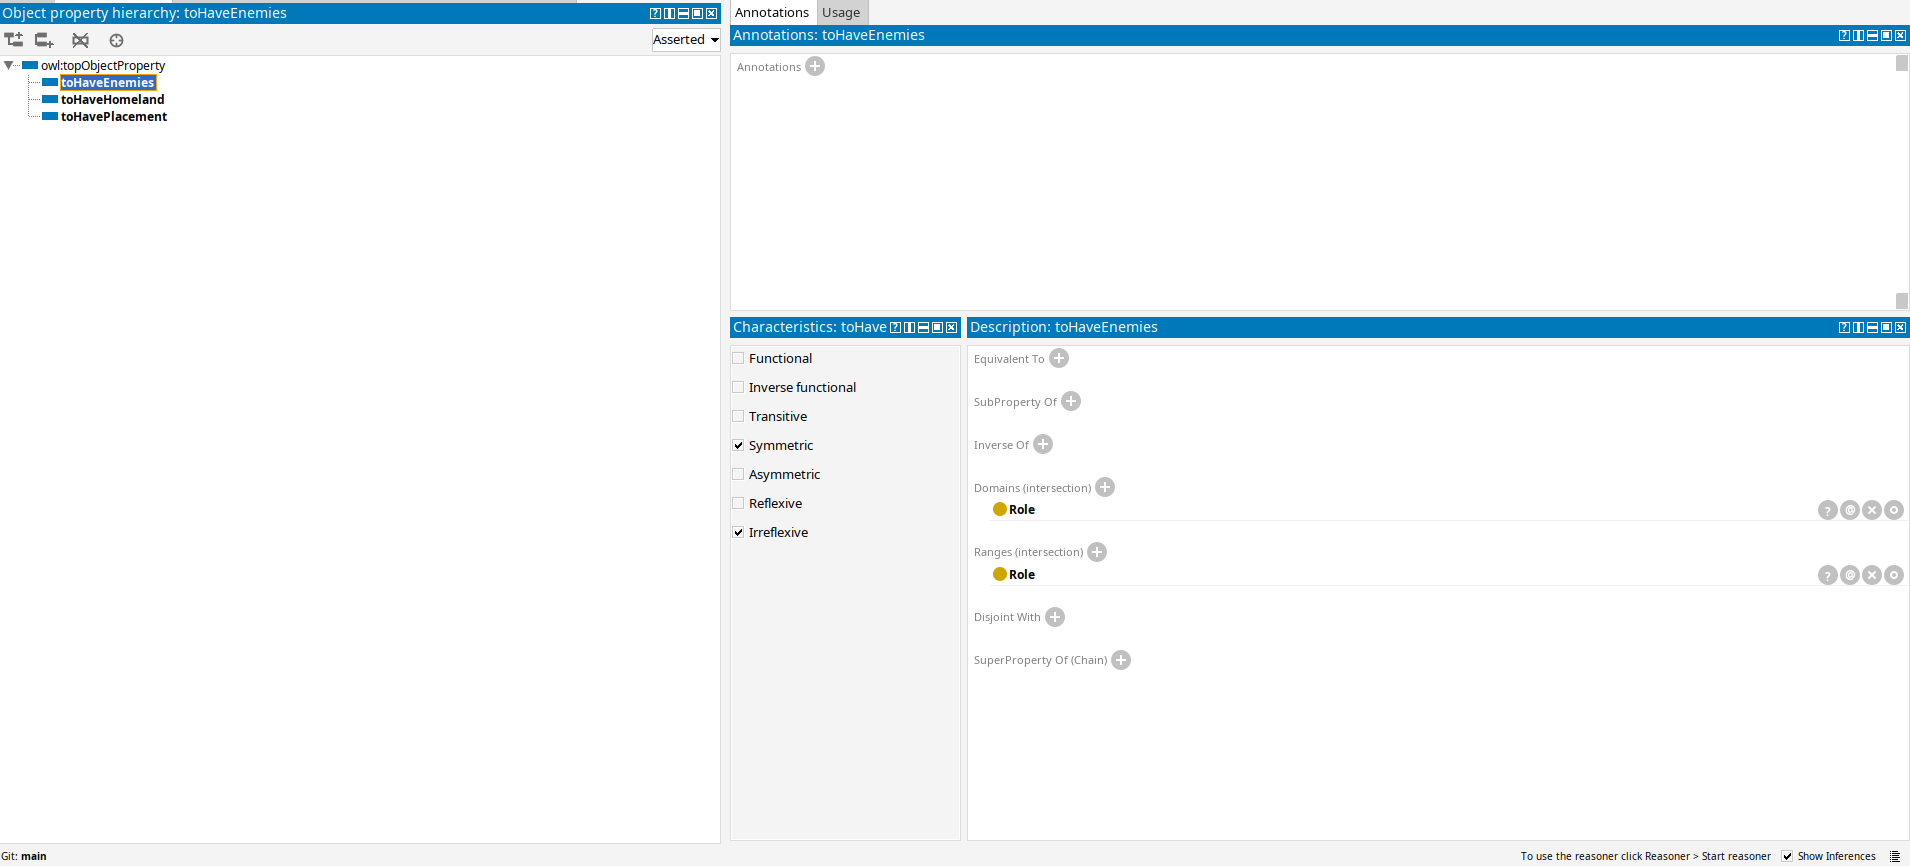
\includegraphics[scale=0.6]{properties}
\end{center}

\mysection{Классы и их объекты}
\begin{center}
	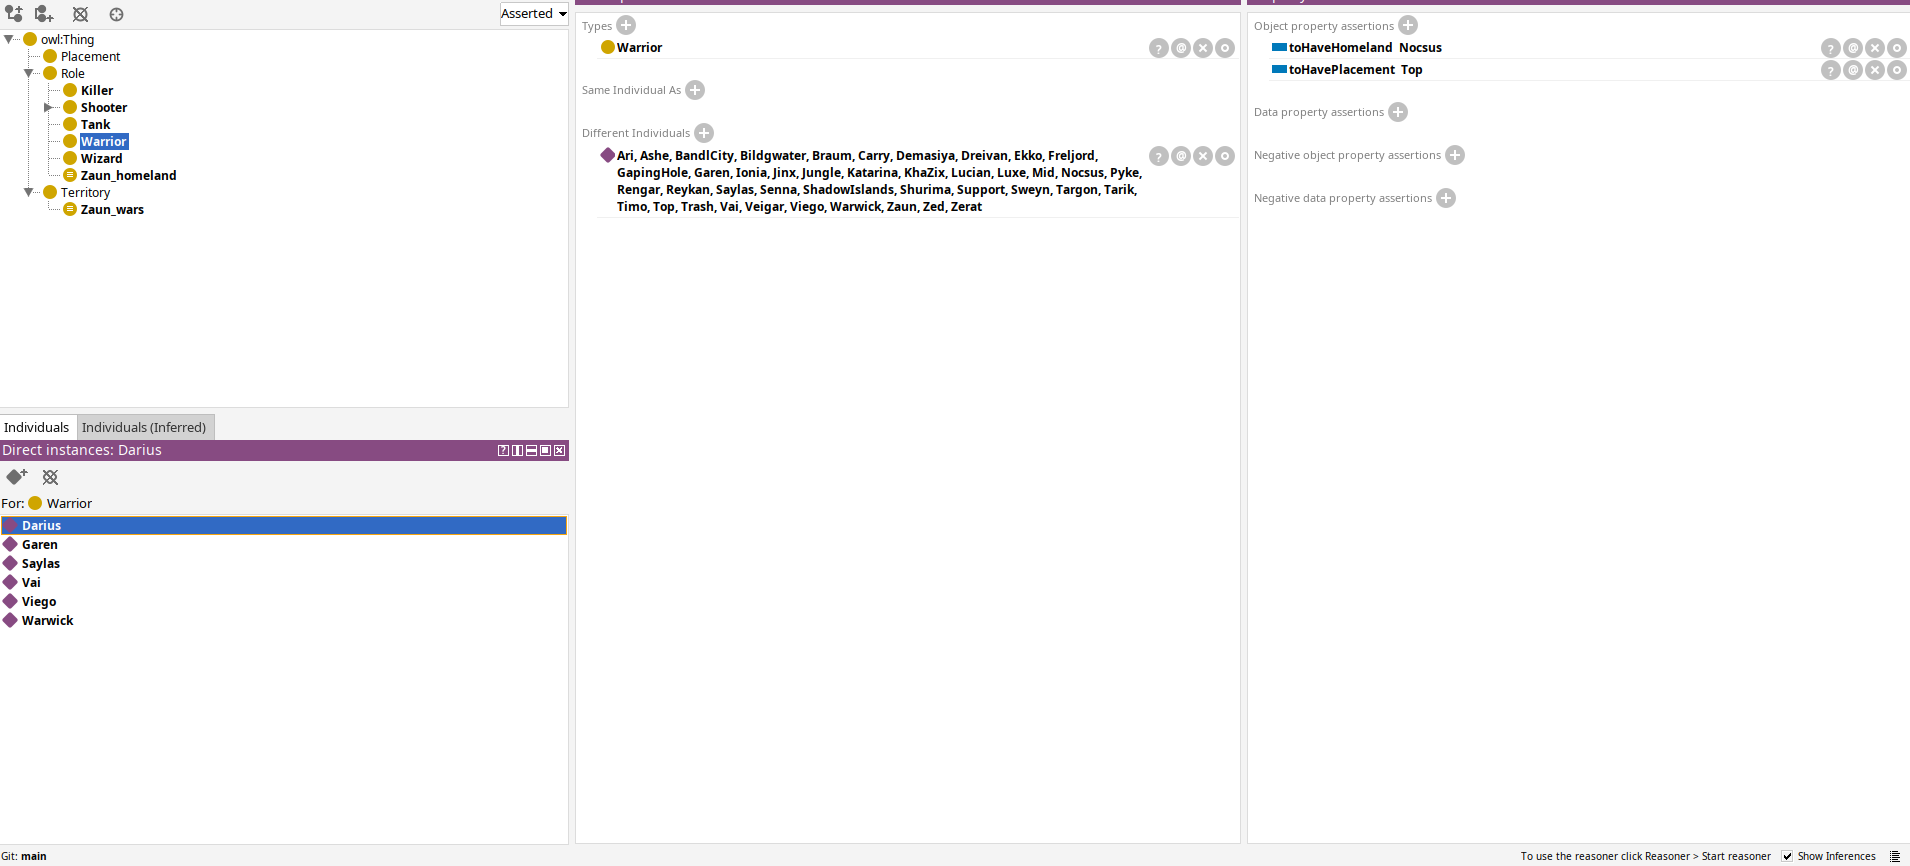
\includegraphics[scale=0.6]{classes_objects}
\end{center}]

\mysection{Запрос Protege}
\begin{center}
	
\includegraphics[scale=0.6]{request_protege}
\end{center}


\newpage
\mysection{Вывод}
Мы познакомились с основными концепциями баз знаний и онтологий, освоили язык Prolog и редактор онтологий Protege. Базы знаний на Prolog позволяют удобно осуществлять резолюцию целей по имеющимся фактам, а система Protege может выявлять несоотвестивия и "скрытую информацию" в разработанных онтологиях.
\end{document}